\section{Syntactic translation}

\begin{definition}[\textit{Transducer}]
    The transducer is an automaton that can produce output via an output function. 
\end{definition}
\begin{definition}[\textit{Translation}]
    The translation is the correspondence between two texts that have the same meaning in two different languages: the given text language is called source, and it's denoted by $\Sigma$ while the other language is called target, and it's denoted by $\Delta$. 
\end{definition}
\begin{definition}[\textit{Purely syntactic method}]
    A purely syntactic method is a method that applies local transformations to the source text, without considering its meaning. 
\end{definition}
The translation grammar is a purely syntactic translation method that uses pushdown transducers on top of a parsing method. 
The translation regular expression is a purely syntactic translation method that uses a finite transducer enriched with an output function. 
\begin{definition}[\textit{Syntax directed method}]
    A syntax directed method is a semiformal approach based on a combination of syntax rules and semantic functions. 
\end{definition}
\begin{definition}[\textit{Syntax directed semantic translation}]
    The syntax directed semantic translation is a semiformal approach based on a combination of syntax rules and semantic functions
\end{definition}
\begin{definition}[\textit{Syntactic representation}]
  The syntax directed semantic translation is a semiformal approach based on a combination of syntax rules and semantic functions
\end{definition}
The procedure for syntax-directed semantic translation involves the following steps:
\begin{enumerate}
    \item Define a set of attributes for nonterminals in the program.
    \item Establish a set of semantic equations governing how attributes are evaluated.
    \item Specify the order in which equations should be evaluated.
    \item Construct a parse tree that captures the syntactic structure of the program.
    \item Traverse the tree in the order of attribute evaluation.
    \item Use equations to compute the specified attributes.
\end{enumerate}

\paragraph*{Analogies of Formal Language and translation Theory}
The set of language phrases aligns with the set of pairs (comprising source and destination strings) that characterize the translation relation.

The language grammar transforms into a translation grammar, responsible for generating pairs of phrases.

Similarly, the finite state automaton or pushdown automaton transforms into a transducer automaton or a syntax analyzer, computing the translation relation.

\subsection{Translation relation and function}
Translation can be defined formally as a binary relation between the source and the target universal languages, denoted as $\Sigma^{*}$ and $\Delta^{*}$, respectively. 
This relation is essentially a function whose domain is a subset of the Cartesian product $\Sigma^{*} \times \Delta^{*}$.
A translation relation $\rho$ is a set of pairs of strings $\left( x, y \right)$ where $x \in \Sigma^{*}$, $y \in \Delta^{*}$, satisfying:
\[ \rho = \left\{ \left( x, y \right),\dots \right\} \subseteq \Sigma^{*} \times \Delta^{*} \]
Here, $y$ is the image (or translation, destination) of the source string $x, $ and they correspond to each other.
Given a translation relation $\rho$, the source and target languages $L_1$ and $L_2$ are defined as:
\[L_1 = \left\{ x \in \Sigma^{*} | \exists y \in \Delta^{*} \textnormal{ such that } \left( x, y \right) \in \rho \right\}\]
\[L_2 = \left\{ y \in \Delta^{*} | \exists x \in \Sigma^{*} \textnormal{ such that } \left( x, y \right) \in \rho \right\}\]
Alternatively, translation can be formalized using the set of all images of a source string, defining a function $\tau$ that maps each source string to the set of corresponding target strings:
\[\tau: \Sigma^{*} \rightarrow \wp \left( \Delta^{*} \right)\]
\[\tau(x) = \left\{ y \in \Delta^{*} | \left( x, y \right) \in \rho \right\}\]
The union of the application of the function $\tau$ to all source strings is the target language $L_2$:
\[ L_2 = \bigcup_{x \in L_1} \tau(x) \]
The translation relation $\rho$ is partially defined, as some strings in the source alphabet might lack a translation in the target alphabet.
To make the function total, a special value, \texttt{error}, is introduced where the application of the function $\tau$ to a string $x$ is undefined.
In cases where each source string has at most one image, the translation function is defined as:
\[ \tau : \Sigma^{*} \rightarrow \Delta^{*} \]
This case is crucial for defining the inverse translation $\tau^{-1}$:
\[ \tau^{-1} : \Delta^{*} \rightarrow \wp\left( \Sigma^{*} \right) \qquad \tau^{-1}(y) = \left\{ x \in \Sigma^{*} | y \in \tau(x) \right\} \]
Similarly, the inverse translation relation $\rho^{-1}$ is obtained by swapping the corresponding source and target strings:
\[ \rho^{-1} = \left\{ \left( y, x \right) | \left( x, y \right) \in \rho \right\} \]
The mathematical properties of $\tau$ give rise to different types of translations:
\begin{enumerate}
    \item \textit{Total}: every source string has one or more images.
    \item \textit{Partial}: one or more source strings lack any image.
    \item \textit{Single-valued}: no string has two distinct images.
    \item \textit{Multivalued}: one or more source strings have more than one image.
    \item \textit{Injective}: distinct source strings have distinct images. 
        An alternative definition is that every target string corresponds to at most one source string, making the inverse translation $\tau^{-1}$ single-valued.
    \item \textit{Surjective}: the image of the translation coincides with the range; every string over the target alphabet is the image of at least one source string.
        In this case, the inverse translation $\tau^{-1}$ is total.
    \item \textit{Bijective}: the translation is both injective and surjective. 
        Only in this case is the inverse translation bijective as well.
\end{enumerate}

\subsection{Transliteration}
Transliteration, also known as alphabetic homomorphism, represents the most straightforward type of translation.
In this process, each source character is transliterated into a target character or string.
The translation defined by an alphabetic homomorphism is single-valued, although this property may not necessarily extend to the inverse function.
Consider any Greek letter, denoted as $x$. Then, for the inverse transliteration:
\[ h^{-1}\left( x \right) = \left\{ \alpha, \dots, \omega \right\} \]
If the homomorphism erases a letter (mapping it to the empty string), the inverse translation becomes multivalued.
This is because any string composed of erasable characters can be inserted at any position in the text. 
If the inverse function is also single-valued, the transliteration becomes bijective, allowing the reconstruction of the source string from a given target string.
Transliteration transforms a letter into another without considering the occurrence context.

\paragraph*{Purely Syntactic Translation}
In the context of a source language defined by a grammar, every syntactic component (e.g., a subtree) of the source language is individually mapped to an equivalent component in the target language.
\begin{definition}[\textit{Translation grammar}]
    A translation grammar $G_T = \left( V, \Sigma, \Delta, P, S \right)$ is a context-free grammar with a terminal alphabet $C \subseteq \Sigma^{*} \Delta^{*}$ of pairs $\left( u, v \right)$ of source/target strings, also expressed as fractions $\frac{u}{v}$.
\end{definition}
\begin{definition}[\textit{Translation relation}]
    The translation relation $\rho_G$ defined by grammar $G_\tau$ is:
    \[ \rho_{G_\tau}  = \left\{ \left( x, y \right) | \exists , z \in L\left( G_\tau \right) \land x = h_\Sigma \left( z \right) \land y = h_\Delta \left( z \right) \right\} \]
    where $h_\epsilon : C \rightarrow \Sigma$ and $h_\Delta : \rightarrow \Delta$ are the homomorphism that map each pair $\left( u, v \right)$ to the corresponding source/target string.
\end{definition}

\subsection{Ambiguity of source grammar and translation}
As previously observed, when the source grammar is ambiguous, a sentence may have two distinct syntax trees, each corresponding to a different target syntax tree. 
Even in cases where the source grammar is unambiguous, the translation can still be multivalued if different target rules are associated with the same source rule in the translation scheme.
\begin{property}[Unambiguity conditions for translations]
    Let $G_\tau = \left( G_1, G_2 \right)$ be a translation grammar such that the source grammar $G_1$ is unambiguous, and that no two rules of target grammar $G_2$ correspond to the same rule of source grammar $G_1$.
\end{property}
When these conditions are satisfied, the translation specified by grammar $G_\tau$ is single-valued, ensuring the definition of a valid translation function.

\subsection{Translation grammar and pushdown automata}
Similar to the recognizer for context-free grammar, a transducer implementing a translation grammar necessitates a stack of unbounded length.
A pushdown transducer, also known as an IO automaton, extends the concept of a pushdown automaton by allowing the output of zero or more characters at each move.

A IO automaton is represented by a $8$-tuple $\left( Q, \Sigma, \Gamma, \Delta, \delta, q_0, Z_0, F \right)$:
\begin{itemize}
    \item $Q$ is a finite set of states.
    \item $\Sigma$ is the source alphabet (input). 
    \item $\Gamma$ is the pushdown stack alphabet. 
    \item $\Delta$ is the target alphabet (output). 
    \item $\delta$ is the state transition and output function: 
        \[\delta : Q \times \left( \Sigma \cup \left\{ \varepsilon \right\} \right) \times \Gamma \rightarrow Q \times \Gamma^{*} \times \Delta^{*}\]
    \item $q_0 \in Q$ is the initial state. 
    \item $Z_0 \in \Gamma$ is the initial stack symbol. 
    \item $F \subseteq Q$ is the set of final states. 
\end{itemize}
The meaning of the function is as follows: if the current state, input character, and stack top are respectively: 
\[ q^{'}, a, Z \]
and it holds: 
\[ \delta\left(q^{'}, a, Z\right) = \left( q^{{''}}, \gamma, y \right) \]
then the automaton reads $a$ from the input and $Z$ from the stack top, enters the state $q^{{''}}$, pushes the string $\gamma$ onto the stack, and outputs the string $y$.
If the automaton recognizes the string by an empty stack, then the set of final states coincides with $Q$.
The underlying automaton of the translator is obtained by removing the target alphabet symbols and the output string actions from the definitions.

\paragraph*{Instantaneous configuration}
The instantaneous configuration of the pushdown transducer is defined as a $4$-tuple $\left( q, y, \eta, z \right) \in \left( Q \times \Sigma^{*} \times \Gamma^{*} \times \Delta^{*} \right)$ where:
\begin{itemize}
    \item $q$ is the current state. 
    \item $y$ is the remaining portion (suffix) of the source string $x$ to be read. 
    \item $\eta$ is the stack content. 
    \item $z$ is the string written to the output tape, up to the current configuration. 
\end{itemize}

\paragraph*{Moves}
When a move is executed, a transition from a configuration to the next one occurs, denoted as: 
\[ \left( q, x, \eta, \omega \right) \mapsto \left( p, y, \lambda, z \right)\]
A computation is a chain of zero or more transitions, denoted by $\overset{*}{\mapsto}$.
\begin{table}[H]
    \centering
    \begin{tabular}{c|c|c}
        \textbf{Current configuration}      & \textbf{Next configuration}               & \textbf{Applied move}                                                                           \\ \hline                                                                                                                                                                        
        $\left( q, ax, \eta Z, z \right)$   & $\left( p, x, \eta \gamma, z y \right)$   & reading move $\delta\left( q, a, Z \right) = \left( p, \gamma, y \right)$                       \\
        $\left( q, ax, \eta Z, z \right)$   & $\left( p, ax, \eta\gamma, zy \right)$    & spontaneous move $\delta\left( q, \varepsilon, Z \right) = \left( p, \gamma, y \right)$
    \end{tabular}
\end{table}
The initial configuration and string acceptance conditions are the same as described for pushdown automata, and the computed translation $\tau$ is defined as follows (assuming that the acceptance condition is by a final state):
\[ \tau\left( x \right) = z \Leftrightarrow \left( q_0, x, Z_0, \varepsilon \right) \overset{*}{\mapsto} \left( q, \varepsilon, \lambda, z \right) \quad \textnormal{with } q \in F, \lambda \in \Delta^{*} \]

\subsection{From translation grammar to pushdown transducer}
Translation schemes and pushdown transducers are two models for representing language transformations: the former is suitable for specifying the translation, while the latter is suitable for its implementation.
\begin{property}[Equivalence of translation grammar and pushdown transducer]
    A translation relation is defined by a translation grammar or scheme if, and only if, it is computed by a (eventually nondeterministic) pushdown transducer.
\end{property}

\paragraph*{Normalization of Translation Rules}
To simplify the rules, the following hypotheses are made for the source/target pairs $\frac{u}{v}$ occurring in the rules, where $u \in \Sigma^{*}$ and $v \in \Delta^{*}$:
\begin{enumerate}
    \item For any pair $\frac{u}{v}$ it holds $|u| \leq 1$: 
        \begin{itemize}
            \item The source $u$ is a single character $a \in \Sigma$ or the empty string $\varepsilon$.
            \item The rule $\frac{a_1 a_2}{v}$ can be replaced by $\frac{a_1}{v}\frac{a_2}{\varepsilon}$.
        \end{itemize}
    \item No rule may contain the following substrings:
        \[ \dfrac{\varepsilon}{v_1} \dfrac{a}{v_2} \quad \text{or} \quad \dfrac{\varepsilon}{v_1} \dfrac{\varepsilon}{v_2} \]
        with $v_1, v_2 \in \Delta^{*}$. 
        If such combinations are present in a rule, they can be respectively replaced by the equivalent pairs: 
        \[ \dfrac{a}{v_1 v_2} \quad \text{or} \quad \dfrac{\varepsilon}{v_1 v_2} \]
\end{enumerate}

\paragraph*{Predictive pushdown transducer construction algorithm}
Let $C$ represent the set of pairs, including those of the form $\frac{\varepsilon}{v}$ with $v \in \Delta^+$ and $\frac{b}{w}$ with $b \in \Sigma$ and $w \in \Delta^{*}$, occurring in some rule of the translation grammar. 
Initially, the stack contains the axiom $S$, and the reading head is positioned at the first character of the source string. 
At each step, the automaton non-deterministically selects an applicable rule and performs the corresponding move. 
It's important to note that this automaton doesn't necessarily require states, although they may be introduced later to enhance its execution.
\begin{table}[H]
    \centering
    \resizebox{\textwidth}{!}{%
    \begin{tabular}{c|c|c|c}
    \textbf{$\#$} & \textbf{Rule}                                                                                                                                           & \textbf{}                                                                                                                 & \textbf{Comment}                                                                                                                          \\ \hline
    1             & \makecell[l]{$A \rightarrow \frac{\varepsilon}{v}BA_1\dots A_n$ \\ $n \geq 0$ \\ $v \in \Delta^{+}, B \in V$ \\ $A_i \in \left( C \cup V \right)$}      & \makecell[l]{if $top=A$ then write($v$) \\ pop \\ push $A_n \dots A_1B$}                                                  & \makecell[l]{emit the string $v$ \\ push on stack the prediction string $BA_1 \dots A_n$}                                                 \\ \hline
    2             & \makecell[l]{$A \rightarrow \frac{b}{w}BA_1\dots A_n$ \\ $n \geq 0$ \\ $w \in \Delta^{*}, b \in \Sigma$ \\ $A_i \in \left( C \cup V \right)$}           & \makecell[l]{if $cc=b \land top=A$ then write($w$) \\ pop \\ push $A_n \dots A_1$ \\ advance the reading head}            & \makecell[l]{char $b$ was next expected and has been read \\ emit the target string $w$ \\ push the prediction string $A_1 \dots A_n$}    \\ \hline
    3             & \makecell[l]{$A \rightarrow BA_1\dots A_n$ \\ $n \geq 0$ \\ $w \in \Delta^{*}, b \in \Sigma$ \\ $A_i \in \left( C \cup V \right)$}                      & \makecell[l]{if $top=A$ then pop \\ push $A_n \dots A_1B$}                                                                & push the prediction string $BA_1 \dots A_n$                                                                                               \\ \hline
    4             & \makecell[l]{$A \rightarrow \frac{\varepsilon}{v}$ \\ $v \in \Delta^{+}$}                                                                               & \makecell[l]{it $top=A$ then write($v$) \\ pop}                                                                           & emit the string $v$                                                                                                                       \\ \hline
    5             & $A \rightarrow \varepsilon$                                                                                                                             & \makecell[l]{if $top=A$ then pop}                                                                                         &                                                                                                                                           \\ \hline
    6             & \makecell[l]{for every pair \\ $\frac{\varepsilon}{v} \in C$}                                                                                           & \makecell[l]{if $top=\frac{\varepsilon}{v}$ then write($v$) \\ pop}                                                       & \makecell[l]{the past prediction $\frac{\varepsilon}{v}$ is now \\ completed by writing $v$}                                              \\ \hline
    7             & \makecell[l]{for every pair \\ $\frac{b}{w} \in C$}                                                                                                     & \makecell[l]{if $cc=b \land top=\frac{b}{w}$ then write($w$) \\ pop \\ advance the reading head}                          & \makecell[l]{the past prediction $\frac{b}{w}$ is now \\ completed by writing $w$}                                                        \\ \hline
    8             &                                                                                                                                                         & \makecell[l]{if $cc=\dashv \land$ stack is empty \\ then accept and halt}                                                 & the string has been translated                
    \end{tabular}%
    }
\end{table}
\begin{itemize}
    \item Rows $1, 2, 3, 4, 5$ are applicable when the stack top is a nonterminal symbol.
        In case $2$, if the right part begins with a source terminal, the move is conditioned by its presence in the input string.
    \item Rows $1, 3, 4, 5$ initiate spontaneous moves, which do not shift the reading head.
    \item Rows $6, 7$ come into play when the stack top is a pair.
        If the pair contains a source character (row $7$), it must match the current input character.
        If the pair contains a target string (rows $6, 7$), the latter is output.
    \item Finally, row $8$ acknowledges the string if the stack is empty, and the current character indicates the end of the input string.
\end{itemize}

\subsection{Syntax analysis with online translation}
A pushdown transducer generated using the predictive pushdown transducer algorithm is often nondeterministic and generally not well-suited for a compiler. 
A more efficient transducer can be directly constructed by transforming a syntactic analyzer into the corresponding syntactic transducer. 
Given a transduction grammar, assuming that the underlying source grammar allows the construction of a deterministic syntax analyzer, the transduction can be computed by directly translating the syntax tree as it is built.
There are two different types of translations depending on the construction of the parser: top-down and bottom-up.
\begin{itemize}
    \item \textit{Top-down analyzer} (LL): a parser of this type can always be transformed into a transducer.
    \item \textit{Bottom-up analyzer} (LR): for a bottom-up analyzer to be transformed into a transducer, every grammar rule must satisfy a special restrictive condition (the write action can only occur at the end of the production).
\end{itemize}

\paragraph*{Top-down deterministic transducer}
Assuming that the source grammar $G_1$ is $\textit{ELL}(k)$ with $k = 1$ (ELL(1)), by completing the corresponding parser with write actions, a deterministic transducer can be constructed.
This approach represents the simplest method for creating a translator. 
The transducer can also be designed using a set of recursive procedures.

\subsection{Regular Translation}
A regular translation expression, also known as a regular translation expression in short, is a regular expression equipped with the union, concatenation, star, and cross operators. It operates on pairs of strings $\left( u, v \right)$, denoted as $\frac{u}{v}$, where the terms $u$ and $v$ may be empty strings belonging to the source and target alphabets, respectively.
\paragraph*{Regular translation expression}
Let $C \subset \Sigma^{*} \times \Delta^{*}$  be the set of pairs $\left( u, v \right)$ occurring in the expression. The Regular Translation (also called rational translation) relation defined by the regular translation expression $e_\tau$ comprises pairs $\left( x, y \right)$ of source and target strings under the following conditions:
\begin{itemize}
    \item There exists a string $z \in C^{*}$ in the regular set defined by the regular translation expression $e_\tau$.
    \item Strings $x$ and $y$ are projections of string $z$ onto the first and second components, respectively.
\end{itemize}
The sets of source and target strings defined by a regular translation expression are regular languages. However, it's crucial to note that not every translation relation, characterized by two regular sets as its source and target languages, can be expressed with a regular translation expression.

\subsection{2I Automaton}
As the set $C$ of pairs occurring in a regular translation expression can be treated as a new terminal alphabet, recognition of the regular language over $C$ can be achieved through a Finite State Automaton.
The concept of a 2I Automaton (two-input automaton) serves as a rigorous method for defining translation and constructing the translation function, enabling the handling of lexical and syntactic translation in a unified manner.
\begin{definition}[2I Automaton]
    A 2I Automaton is a finite automaton with two inputs.
    It is defined by a set of states $Q$, an initial state $Q_0 \in Q$, and a set $F \subseteq Q$ of final states. 
    The transition function $\delta$ is defined as follows:
    \[ \delta : Q \times \left( \Sigma \cup \left\{ \varepsilon \right\} \right) \times \left( \Delta \cup \left\{ \varepsilon \right\} \right) \rightarrow \wp (Q) \]
\end{definition}
An automaton move involves the following actions:
\begin{enumerate}
    \item The automaton enters state $q^{'}$.
    \item If $q^{'} \in \delta(q, a, b)$, the automaton reads $a$ from the source tape and $b$ from the target tape. 
    \item If $q^{'} \in \delta(q, \varepsilon, b)$, the automaton does not read the source tape and reads character $b$ from the target tape. 
    \item If $q^{'} \in \delta(q, \varepsilon,\varepsilon)$, the automaton does not read the source tape and does not read the target tape. 
\end{enumerate}
The automaton recognizes the source and target strings if the computation concludes in a final state after both tapes have been entirely scanned. 
A transition from a state $q_n$ to a state $q_m$ while reading a pair $\left( a, b \right)$ respectively from the source and from the target tape is denoted as $\xrightarrow{\frac{a}{b}}$.
\begin{figure}[H]
  \centering
  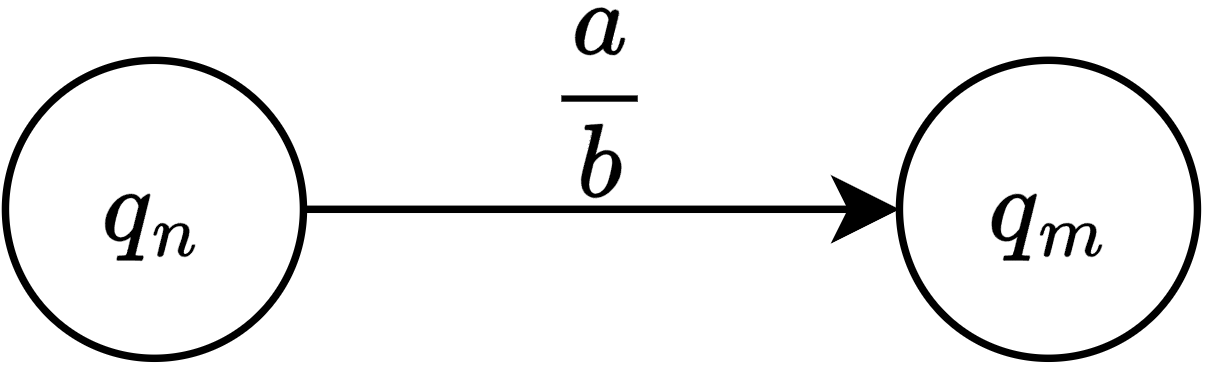
\includegraphics[width=0.25\linewidth]{images/2i.png}
\end{figure}

\paragraph*{Automaton forms}
By projecting the arc labels of a 2I automaton onto the first component, a new automaton with one input tape is obtained.
The symbols on the tape belong to the source alphabet $\Sigma$, and the resulting automaton is subjacent to the original machine.
A 2I automaton in normal form is characterized by the fact that each move reads exactly one character either from the source tape or from the target tape, but not from both.
Arc labels can be of the following types:
\begin{enumerate}
    \item Label $\dfrac{a}{\varepsilon}$ with $a \in \Sigma$ if one character from the source is read.
    \item Label $\dfrac{\varepsilon}{b}$, with $b \in \Delta$, if one character from the target is read.
\end{enumerate}
The families of translation defined by regular translation expressions and by finite (eventually nondeterministic) 2I automata coincide.
\begin{theorem}[Nivat Theorem]
    The Nivat Theorem states the following $4$ conditions are equivalent:

    The translation relation $\rho_\tau$ is defined by a right-linear (or left-linear) translation grammar $G_\tau$.

    The translation relation $\rho_\tau$ is defined by a 2I-automaton.

    The translation relation $\rho_\tau \subseteq \Sigma^{*} \times \Delta^{*}$ is regular.

    There exists and alphabet $\Omega$, a regular language $R$ over $\Omega$ and two alphabetic homomorphism: 
    \[h_1 : \Omega \rightarrow \Sigma \cup \left\{ \varepsilon \right\}\]
    \[h_2 : \Omega \rightarrow \Delta \cup \left\{ \varepsilon \right\}\]
    such that:
    \[ \rho_\tau = \left\{ \left( h_1(z), , h_2(z) \right) | z \in R \right\} \]
\end{theorem}

\subsection{Sequential Transducer}
Sequential transducers are automata used to efficiently compute translations in real-time while reading the input tape. 
Finally, when the input is finished, the automaton may append a finite piece of text that depends on the final state reached.
\begin{definition}[\textit{Sequential transducer}]
    A sequential transducer or IO-automaton $T$ is a deterministic machine defined by a set $Q$ of states, a source alphabet $\Sigma$ and a target alphabet $\Delta$, an initial state $q_0$ and a set $F \subseteq Q$ of final states.
\end{definition}
Furthermore, there are three single-valued functions:
\begin{enumerate}
    \item The state transition function $\delta$ computes the next state.
    \item The output function $\eta$ computes the string to be emitted by a move.
    \item The final function $\phi$ computes the last suffix to be appended to the target string at termination.
\end{enumerate}
The domains and images of these three functions are as follows:
\[ \delta: Q \times \Sigma \rightarrow Q \quad \eta: Q \times \Sigma \rightarrow \Delta^{*} \quad \phi : F \times \left\{ \dashv \right\} \rightarrow \Delta^{*} \]
The graphical representation of the two functions $\delta(q, a) = r$ and $\eta(q, a) = u$ is:
\[ q \xrightarrow{\dfrac{a}{u}} r \]
which means that in the state $q$, while reading character $a$, emits string $u$ and moves to the next state $r$.
The ultimate function $\phi(r, \dashv)$ denotes that upon complete reading of the source string, if the final state is $r$, then the corresponding output string is $v$.
For a source string $x$, the translation $\tau(x)$ computed by the sequential transducer $T$ results from the combination of two strings generated by the output function and the final function:
\[ \left\{ yz \in \Delta^{*} , |dle\vert , \exists  \textnormal{ a computation labelled } \dfrac{x}{y} \textnormal{ ending in } r \in F \land z = \phi\left( r, \dashv \right) \right\} \]
The machine is deemed deterministic because the input automaton $\langle Q, \Sigma, \delta, q_0, F \rangle$ associated with $T$ is deterministic, and both the output and final functions, $\eta$ and $\phi$, are single-valued.
However, the determinism of the underlying input automaton alone does not guarantee that the translation is uniquely determined, as there could be non-unique outputs between two states of the sequential transducer $T$, such as when there are two arcs labeled $\frac{a}{b}$ and $\frac{a}{c}$.

A function computable through a sequential state transducer (IO-automaton) is referred to as a sequential function, and the composition of two sequential functions yields another sequential function.

\paragraph*{Two opposite passes}
In cases where a single-valued translation is specified by a regular translation expression or a 2I automaton, it may not always be feasible to implement the translation using a sequential transducer like a deterministic IO-automaton. 
However, in such scenarios, the translation can be realized through two consecutive (deterministic) sequential passes, each moving in opposite directions while scanning the string:
\begin{enumerate}
    \item A sequential transducer scans \textit{from left to right}, converting the \textit{source string} into an intermediate string.
    \item Another sequential transducer scans the \textit{intermediate string from right to left}, generating the specified target string.
\end{enumerate}